% !TeX spellcheck = russian-aot
\documentclass{article}

\usepackage[vmarginratio=1:1,a4paper,body={6.5in, 9.5in}]{geometry}

\usepackage[T2A]{fontenc}
\usepackage[utf8]{inputenc}
\usepackage[russian]{babel}

\usepackage{amsmath}
\usepackage{amssymb}
\usepackage{amsfonts}
\usepackage{amsthm}
\usepackage{color}

\usepackage{hyperref}
\usepackage{graphicx}

\usepackage{mathtools}
\DeclarePairedDelimiter{\diagfences}{(}{)}
\newcommand{\diag}{\operatorname{diag}\diagfences}

\newcommand{\sign}{\operatorname{sign}}
\DeclarePairedDelimiter{\homd}{\lceil}{\rfloor}

\title{Reaction wheel 1D pendulum}
\author{}
\date{}

\begin{document}

\maketitle
% The Reaction Wheel Pendulum (Block, Atrom, Spong)
%ftp://nozdr.ru/biblio/kolxo3/P/PC/PCtm/Block%20D.,%20Astroem%20K.,%20Spong%20M.%20The%20Reaction%20Wheel%20Pendulum%20(MC,%202007)(ISBN%201598291947)(O)(112s)_PCtm_.pdf

\section{Вывод уравнений движения}

\begin{minipage}[t]{.2\linewidth}
\vspace{0cm}
\centerline{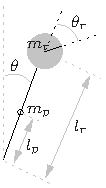
\includegraphics[width=\linewidth]{img/schema}}
\end{minipage}
\begin{minipage}[t]{.8\linewidth}
\vspace{0cm}
\begin{itemize}
    \item $m_p$ - масса маятника
    \item $m_r$ - масса ротора
    \item $l_p$ - расстояние от шарнира до центра масс маятника
    \item $l_r$ - расстояние от шарнира до центра масс ротора
    \item $J_p$ - момент инерции маятника при вращении вокруг центра масс
    \item $J_r$ - момент инерции ротора
    \item $\theta$ - угол маятника относительно вертикали
    \item $\theta_r$ - угол ротора \textbf{относительно маятника}
    \item $\tau$ - момент, прикладываемый к ротору
    \item $C_p$ - коэффициент вязкого трения в шарнире маятника
    \item $C_r$ - коэффициент вязкого трения ротора
\end{itemize}
\end{minipage}

\vspace{5mm}

Кинетическая энергия маятника:
$$
T_p = \frac{1}{2} (m_pl_p^2 + J_p)\dot\theta^2
$$

Кинетическая энергия маховика:
$$
T_r = \frac{1}{2} m_r l_r^2 \dot\theta^2 + \frac{1}{2}J_r (\dot\theta_r+\dot\theta)^2
$$

Общая потенциальная энергия:
$$
P = (m_pl_p + m_r l_r)g \cos\theta
$$

Лагранжиан:
$$
\mathcal{L} = T_p + T_r - P
$$

Введём новые обозначения констант, которые нам уменьшат общее количество закорючек в уравнениях:
\begin{align*}
ml&:=m_p l_p + m_r l_r\\
J &:= J_p + m_p l_p^2 + m_r l_r^2
\end{align*}

Тогда лагранжиан запишется следующим образом:
$$
\mathcal L = \frac{1}{2}J\dot\theta^2 + \frac{1}{2}J_r(\dot\theta_r+\dot\theta)^2 - mlg\cos\theta
$$

Для удобства выпишем все частные производные:
\begin{align*}
\frac{\partial\mathcal L}{\partial\dot\theta_r} &= J_r(\dot\theta_r + \dot\theta)       & \frac{\partial\mathcal L}{\partial\theta_r} &= 0            \\
\frac{\partial\mathcal L}{\partial\dot\theta}   &= (J+J_r)\dot\theta + J_r\dot\theta_r  & \frac{\partial\mathcal L}{\partial\theta}   &= mlg\sin\theta\\
\end{align*}

Напоминалка про уравнения Лагранжа:
$$
\frac{d}{dt}\left(\frac{\partial\mathcal L}{\partial\dot q_i}\right) - \frac{\partial\mathcal L}{\partial q_i} = \tau_i,
$$
где $q$ это обобщённая координата. В нашем случае мы выбираем $q:=(\theta_r, \theta)^\top$.

Тогда уравнения движения примут следующий вид:
\begin{align*}
J_r\ddot\theta_r + J_r\ddot\theta&= - C_r \dot\theta_r + \tau,\\
(J+J_r)\ddot \theta + J_r\ddot\theta_r - mlg\sin\theta &= - C_p \dot\theta.
\end{align*}

Перепишем, оставив вторые производные слева:
$$
\left\{
\begin{array}{l}
\ddot\theta_r = \frac{J+J_r}{J J_r}(\tau - C_r\dot\theta_r) - \frac{mlg}{J}\sin\theta + \frac{C_p}{J}\dot\theta\\
\ddot\theta   = -\frac{\tau}{J} + \frac{ml g}{J}\sin\theta  - \frac{C_p}{J} \dot\theta + \frac{C_r}{J} \dot\theta_r
\end{array}
\right.
$$

Или перепишем в матричной форме:
\begin{equation} \label{eq:mechModel:generalized}
	M\ddot{q} + G(q) =\mathcal{T}(\dot{q},\tau),
\end{equation}
где
\[
	M := \begin{bmatrix} J_r & J_r \\
						 J_r & J_r+J
		 \end{bmatrix},
	\;
	G(q): = \begin{bmatrix} 0 \\ -mlg \sin(q_2) \end{bmatrix},
	\;
	\mathcal{T}(\dot{q},\tau) := \begin{bmatrix} - C_r \dot\theta_r + \tau \\ - C_p \dot\theta \end{bmatrix}.
\]

Наверняка трение в маятнике будет существенно ниже трения в роторе, и вполне возможно, что при этом пренебречь можно будет обоими. 


{\color{blue} Эти уравнения движения полностью совпадают с уравнениями из \href{https://www.ethz.ch/content/dam/ethz/special-interest/mavt/dynamic-systems-n-control/idsc-dam/Research_DAndrea/Cubli/Cubli_IROS2012.pdf}{The Cubli: A Cube that can Jump Up and Balance}, а также с уравнениями из \href{https://dl.acm.org/citation.cfm?id=3019246}{The Reaction Wheel Pendulum} (с точностью до выбора переменных, Åström отсчитывает угол ротора от вертикали). Но Åström в уравнения Лагранжа вставляет моменты $\tau$ и $-\tau$, а я тут вставляются $\tau$ и 0. Подход Острёма интуитивно понятен: если на ротор действует момент $\tau$, то на маятник действует момент $-\tau$. Впрочем, это зависит от выбора репера ($\theta_r$ отсчитывается от вертикали или от маятника). Нечего выбирать неортогональные базисы пространства конфигураций.}


\section{Как выбрать размер маховика?} \label{sec:wheelSize}
Здесь я напишу уравнения движения для обычного коллекторного двигателя, но для бесколлекторных уравнения примерно такие же.
Подадим на клеммы мотора максимально возможное напряжение, для заданного маховика задача состоит в том, чтобы найти максимально возможный угол начального отклонения маятника, при котором разгоняющийся маховик сможет перекинуть маятник через ноль.
Затем будем варьировать размер маховика и смотреть, как будет изменяться максимально возможный угол отклонения.

Заглянем в даташит мотора:
\begin{itemize}
    \item $L$ - индуктивность обмотки
    \item $R$ - сопротивление обмотки
    \item $k$ - torque constant (= back-EMF constant)
\end{itemize}

Добавим в уравнения движения уравнение мотора:
$$
\left\{
\begin{array}{l}
\ddot\theta_r = \frac{J+J_r}{J J_r}(kI - C_r\dot\theta_r)  -\frac{mlg}{J}\sin\theta + \frac{C_p}{J}\dot\theta\\
\ddot \theta  = -\frac{k}{J} I + \frac{mlg}{J}\sin\theta - \frac{C_p}{J} \dot\theta + \frac{C_r}{J} \dot\theta_r\\
\dot I  = \frac{U}{L} - \frac{R}{L}I - \frac{k}{L} \dot\theta_r\\
\end{array}
\right.
$$

Для грубой прикидки размера маховика будем пренебрегать всяким. Индуктивность обмоток мотора очень низкая, поэтому можно сказать, что $I=\frac{U}{R}-\frac{K}{R}\,\dot\theta_r$. Вязкие трения тоже убираем, $C_r=C_p=0$. 

\subsection{Численное решение на основе нелинейной модели}
Итак, у нас есть модель \eqref{eq:mechModel:generalized}. Мы пренебрегаем индуктивностью и рассматриваем модель мотора вида
\[
	\tau = kI = \frac{k}{R}U - \frac{k^2}{R} \dot{\theta}_r.
\]
Перепишем модель \eqref{eq:mechModel:generalized} в виде
\[
	M\ddot{q} = -G(q) - \begin{bmatrix} C_r + \frac{k^2}{R}  & 0 \\ 0 & C_p  \end{bmatrix} \dot{q} + \begin{bmatrix}\frac{k}{R} \\ 0 \end{bmatrix}U.
\]
Выберем начальные условия в виде $q(0)=\begin{bmatrix}0 & -\theta_0 \end{bmatrix}^\top$ и $\dot{q}(0)=\begin{bmatrix} 0 & 0 \end{bmatrix}^\top$. Тогда наша задача может быть сформулирована следующим образом: при заданных параметрах маховика, то есть матрице $M$, найти максимальное значение $\theta_0$, при котором траектория $q_2(t) = \theta(t)$ достигает нуля при входном воздействии $U(t)=-U_{max}$, где $U_{max}$ это максимальное значение управления (напряжения). Минус тут стоит так как момент на маятник создаётся с противоположным знаком по сравнению с моментом на маховике. Эта задача решается численно с использованием матлабовского \texttt{ode45}.

Немного забегая вперёд, результат вычислений приведён на рисунке \ref{fig:rwdiameter}.
\begin{figure}[tb]
\centerline{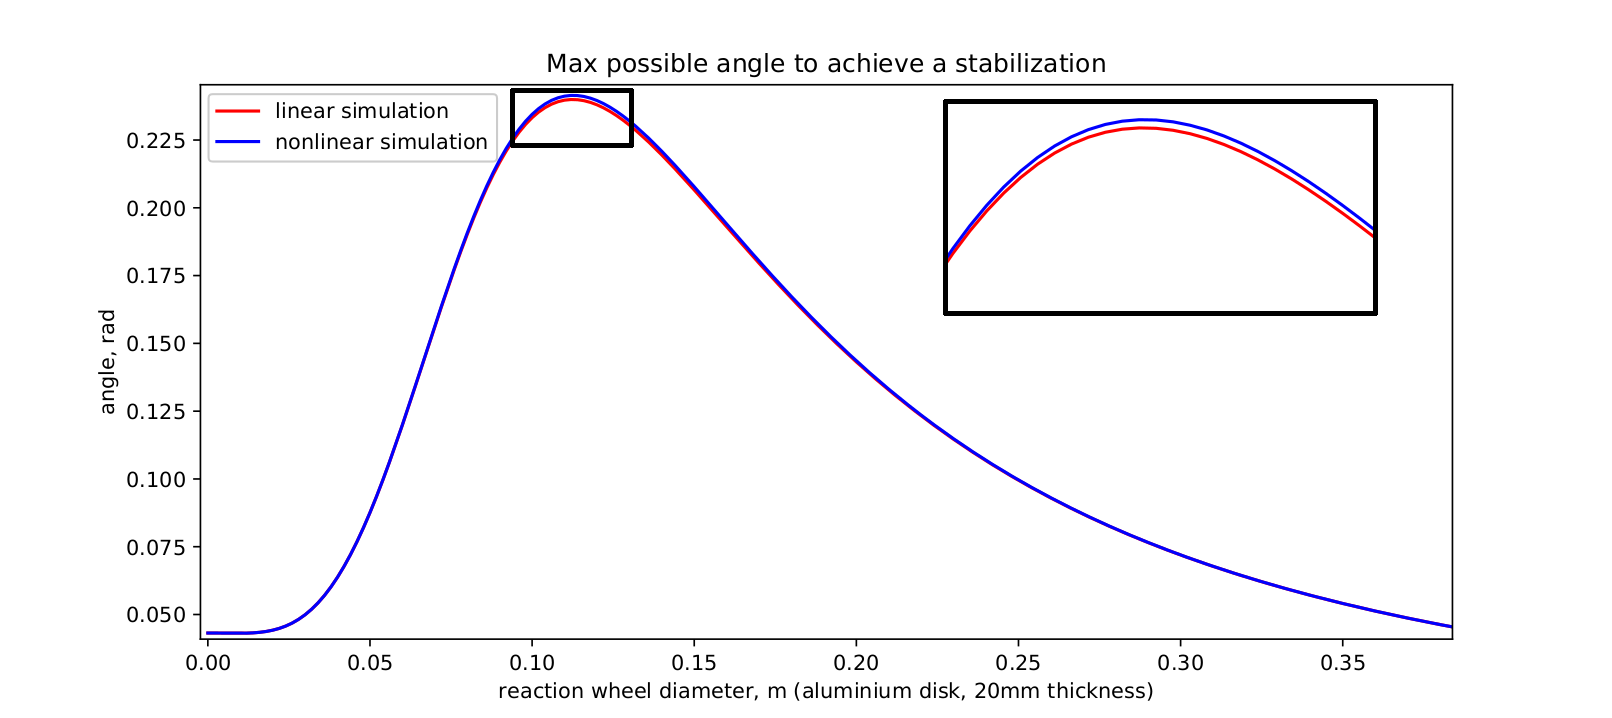
\includegraphics[width=\linewidth]{img/rwsize}}
\caption{Самый выгодный диаметр маховика - 11см, при этом можно будет отклонить маятник на 0.24 радиана.
Видно, что результаты моделирования линеаризованной модели и исходной практически идентичны.
}
\label{fig:rwdiameter}
\end{figure}

\subsection{(Почти) аналитическое решение на основе линеаризации}\label{sec:wheelSize:linear}

На всякий случай проверим правильность запрограммированной нелинейной оптимизации при помощи полуаналитического решения.
Рабочая зона наверняка будет узкой, поэтому заменим синус напрямую на его аргумент. Мысль такая: если будет стабилизироваться линеаризованная модель, то с синусом и подавно маятник встанет. Тогда уравнения движения будут выглядеть следующим образом:
$$
\left\{
\begin{array}{l}
\ddot\theta_r = \frac{J+J_r}{J J_r}(\frac{k\,U}{R} - \frac{k^2}{R}\dot\theta_r)  - \frac{mlg}{J}\theta\\
\ddot \theta  = -\frac{k\,U}{J\,R} + \frac{k^2}{J\,R}\dot\theta_r + \frac{mlg}{J}\theta
\end{array}
\right.
$$

Ну или в матричном виде: 
$$
\frac{d}{dt}\begin{pmatrix}\theta \\ \dot\theta \\ \dot\theta_r \end{pmatrix} = A \begin{pmatrix}\theta \\ \dot\theta \\ \dot\theta_r \end{pmatrix} + B U,
$$
где:
$$
A= \begin{pmatrix} 0 & 1 & 0 \\ \frac{mlg}{J} & 0 & \frac{k^2}{JR} \\ -\frac{mlg}{J} & 0 & -\frac{(J+J_r)k^2}{J\,J_r\,R} \end{pmatrix},
\qquad 
B=\begin{pmatrix}0\\ -\frac{k}{JR} \\ \frac{(J+J_r)k}{J\,J_r\,R} \end{pmatrix}.
$$

На всякий случай выпишем характеристический многочлен:
$$\chi(\lambda) = -\lambda^3 - \frac{k^2(J_r+J)}{J_rJR}\,\lambda^2 + \frac{mlg}{J}\,\lambda+\frac{mlgk^2}{J_rJR}.$$
Он имеет три различных вещественных корня, два из них отрицательных, один положительный. В этом легко убедиться:
$$
\chi(0)>0,\quad \lim\limits_{\lambda\rightarrow-\infty}\chi(\lambda)=+\infty,\quad \lim\limits_{\lambda\rightarrow+\infty}\chi(\lambda)=-\infty,\quad\chi\left(-\sqrt{\frac{mlg}{J}}\right) = -\frac{mlg k^2}{J^2 R}<0.
$$
Аргумент в последнем неравенстве вылез из желания сократить кубическое и линейное слагаемые многочлена.
Положительное собственное число говорит о том, что в отсутствие управления система у нас неустойчива.
Поскольку у нас три различных вещественных корня, то матрица $A$ будет иметь полный набор вещественных собственных векторов, соответственно можно произвести её спектральное разложение $A = V \Lambda V^{-1}$, где $V$ - это матрица, составленная из трёх собственных векторов-столбцов, а $\Lambda=\diag{\lambda_1, \lambda_2, \lambda_3}$ - диагональная матрица собственных чисел.
На всякий случай давайте скажем, что $V$ можно записать в следующем виде:
$$
V=\begin{pmatrix}
\frac{k^2}{JR}              & \frac{k^2}{JR}              & \frac{k^2}{JR}               \\
\frac{k^2}{JR}\lambda_1     & \frac{k^2}{JR}\lambda_2     & \frac{k^2}{JR}\lambda_3      \\
\lambda^2_1 - \frac{mlg}{J} & \lambda^2_2 - \frac{mlg}{J} & \lambda^2_3 - \frac{mlg}{J} 
\end{pmatrix}.
$$
Конкретно это нам не очень поможет, так как собственные числа мы явно не выписывали. Перемножая $(A-\lambda_iE)\times V$, мы получим вектор нулей, так как в последней координате будет стоять характеристический многочлен.

Наша задача найти зону устойчивости нашего диффура. Для начала сделаем замену переменной $x=Vy$.
Не умаляя общности, будем считать, что $\lambda_1>0>\lambda_2>\lambda_3$.
Тогда наше уравнение $\dot x = Ax + BU$ перепишется как $V\dot y = AVy + BU$. Домножим слева на $V^{-1}$: 
$$
\dot y = V^{-1}AVy + V^{-1}BU = \Lambda y + V^{-1}BU.
$$
Эта замена переменной сделана для того, чтобы зона устойчивости имела красивое выражение, будучи разложенной на независимые переменные.
В силу диагональности новой матрицы системы, вторая и третья координата $y$ нас не интересуют вообще, нам интересна координата, которая соответствует положительному собственному числу.
Обозначим через $b_1$ первую координату вектора $V^{-1}BU$ (напоминаю, что у нас напряжение $U$ постоянно).
Вполне очевидно, что зона устойчивости этого диффура представляет собой пространство между двумя плоскостями $\left(-\frac{|b_1|}{\lambda_1}, \frac{|b_1|}{\lambda_1} \right) \times \mathbb R \times \mathbb R$.

Это прекрасно, но нас интересует устойчивость в терминах изначальных переменных.
Если мы сделаем обратное преобразование, то в пространстве $x$ зона устойчивости также будет заключена между двумя параллельными плоскостями.
Плоскости будут наклонными, т.к. мы себе можем позволить больший угол отклонения, если правильно подкрутить начальные скорости.
Но нас интересует конкретный случай, когда обе скорости нулевые. Самый простой способ это посчитать - это взять луч с направляющим вектором $(1,0,0)$, преобразовать его при помощи $V^{-1}$,
пересечь с плоскостью $y_1 = \frac{|b_1|}{\lambda_1}$, а затем точку пересечения обратно преобразовать при помощи $V$.

Решаем численно, так как очень уж громоздко выписывать собственные вектора символьно.
Картинка~\ref{fig:rwdiameter} показывает максимальный угол, из которого можно стабилизировать маятник, для данного диаметра маховика.
Решение практически совпадает с нелинейной оптимизацией.


%\begin{figure}[tb]
%	\centerline{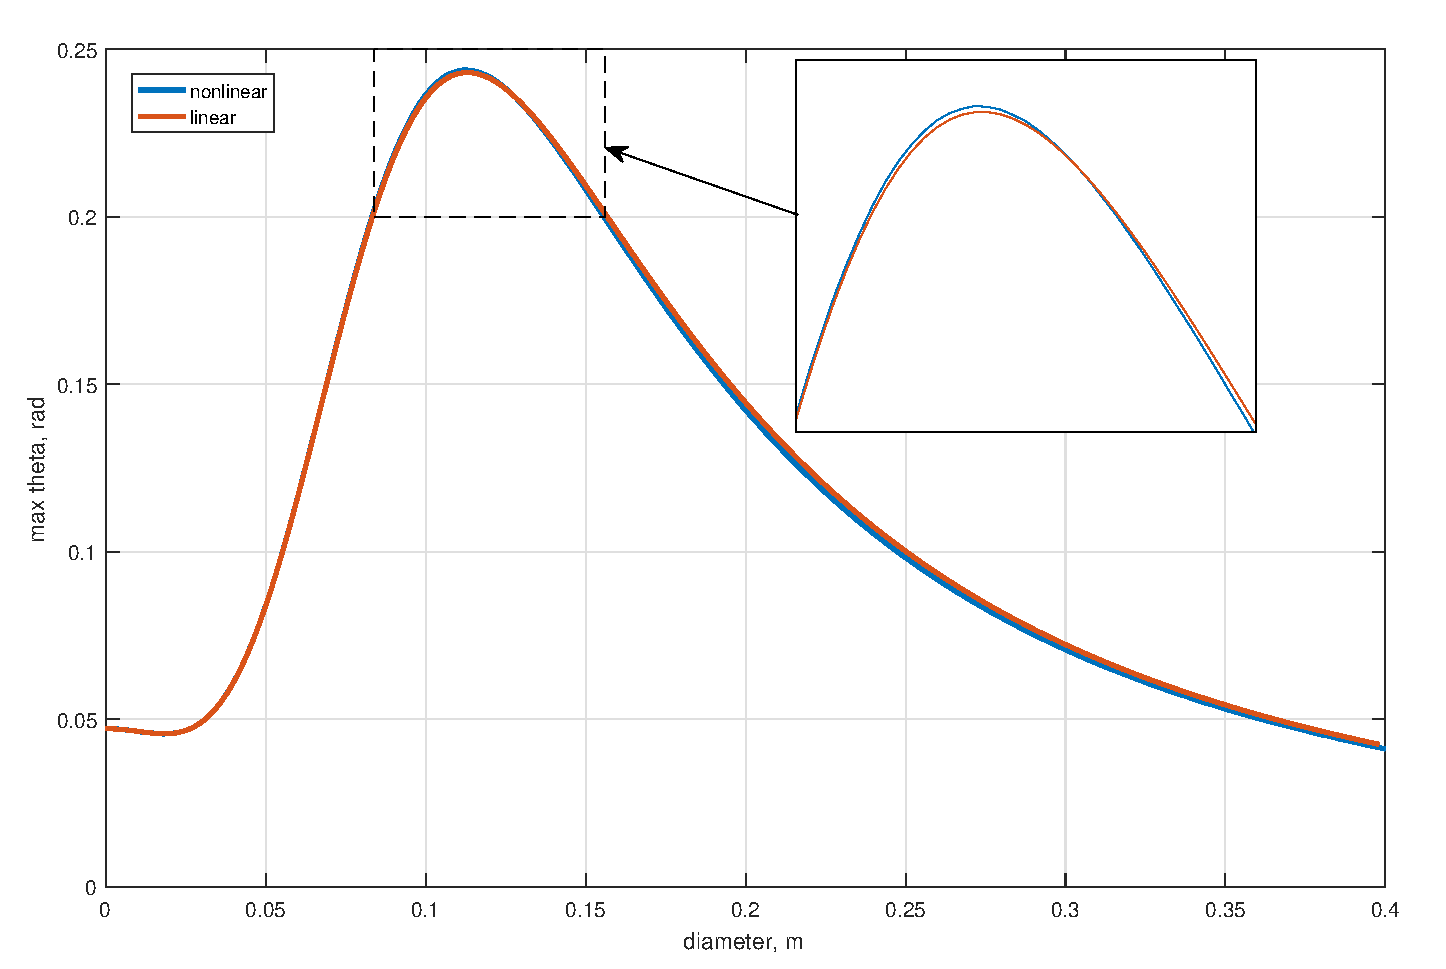
\includegraphics[width=.6\linewidth]{img/RWcomparison}}
%	\caption{Видно, что результаты практически идентичны.}
%	\label{fig:rwdiameter:comparison}
%\end{figure}

\iffalse

\newpage
\section{Давайте разбираться с моментами}
Силы тяжести нет, трения нет, все моменты инерции равны единице.
$$
q_v = q_p + \theta
$$

\subsection{Неподвижный репер}

Возьмём в качестве обобщённых координат $\theta$ и $q_v$. Тогда лагранжиан запишется так:
$$
\mathcal{L} = \frac{1}{2} \dot \theta^2 + \frac{1}{2}\dot q^2_v
$$

Для удобства выпишем все частные производные:
\begin{align*}
\frac{\partial\mathcal L}{\partial\dot q_v} &= \dot q_v   && \frac{\partial\mathcal L}{\partial q_v} = 0\\
\frac{\partial\mathcal L}{\partial\dot\theta} &= \dot\theta && \frac{\partial\mathcal L}{\partial\theta} = 0\\
\end{align*}

Выпишем уравнения Лагранжа:

\begin{align*}
\frac{d}{dt}\left(\frac{\partial\mathcal L}{\partial\dot q_v}\right) - \frac{\partial\mathcal L}{\partial q_v} = \ddot q_v = \tau\\
\frac{d}{dt}\left(\frac{\partial\mathcal L}{\partial\dot \theta}\right) - \frac{\partial\mathcal L}{\partial \theta} = \ddot\theta = -\tau\\
\end{align*}

\subsection{Вращающийся репер}

Возьмём в качестве обобщённых координат $\theta$ и $q_p$. Тогда лагранжиан запишется так:
$$
\mathcal{L} = \frac{1}{2} \dot \theta^2 + \frac{1}{2}(\dot q_p+\dot\theta)^2
$$

Для удобства выпишем все частные производные:
\begin{align*}
\frac{\partial\mathcal L}{\partial\dot q_p} &= \dot q_p + \dot\theta && \frac{\partial\mathcal L}{\partial q_p} = 0\\
\frac{\partial\mathcal L}{\partial\dot\theta} &= 2\dot\theta +\dot q_p &&  \frac{\partial\mathcal L}{\partial\theta} = 0\\
\end{align*}

Выпишем уравнения Лагранжа. Предположим, что я не знаю действующих моментов, обозначу их через $x$ и $y$, буду их искать так, чтобы уравнения совпали с уравнениями из предыдущего параграфа.

\begin{align*}
\frac{d}{dt}\left(\frac{\partial\mathcal L}{\partial\dot q_p}\right) - \frac{\partial\mathcal L}{\partial q_p}= \ddot q_p + \ddot\theta = x\\
\frac{d}{dt}\left(\frac{\partial\mathcal L}{\partial\dot \theta}\right) - \frac{\partial\mathcal L}{\partial \theta}= 2\ddot\theta +  \ddot q_p   = y\\
\end{align*}

Перепишем наши уравнения движения следующим образом:

\begin{align*}
\ddot q_p = 2x - y\\
\ddot\theta = y - x
\end{align*}

Очевидно, что если $\ddot q_v = \tau$, то $\ddot q_p = 2\tau$, поскольку $q_v = q_p + \theta$, а $\ddot\theta = -\tau$. Запишем уравнения для $x$ и $y$:

\begin{align*}
\ddot q_p = 2x - y = 2\tau\\
\ddot\theta = y - x = -\tau
\end{align*}

Решением является $x=\tau, y=0$. ЧТД.

\fi

\section{Стабилизация}

\subsection{Контур тока}
У нас есть хороший усилитель и быстрый контур тока. Так что мы можем считать, что управляем моментом напрямую и компенсируем противо-ЭДС. Тогда в модели системы мы положим $\tau=kI$ и будем считать, что $I$ это наш сигнал управления.  
\subsection{LQR}
Линеаризованная модель с контуром тока имеет вид
\[
	\dot{X} = A X + B I,
\]
где, пренебрегая вязким трением,
\[
X = \begin{pmatrix}\theta \\ \dot\theta \\ \dot\theta_r \end{pmatrix},
\qquad 
A= \begin{pmatrix} 0 & 1 & 0 \\ \frac{mlg}{J} & 0 & 0 \\ -\frac{mlg}{J} & 0 & 0 \end{pmatrix},
\qquad 
B=\begin{pmatrix}0\\ -\frac{k}{J} \\ \frac{(J+J_r)k}{J\,J_r} \end{pmatrix}.
\]

Сюда надо будет добавить построение LQR для стабилизации.

\subsection{Ошибка калибровки датчика положения}\label{sec:calib}

Итак, если мы записываем LQR, то у нас система будет вести себя как $\dot X = A X - B K X$, где
$
K= \begin{pmatrix} k_1 & k_2 & k_3 \end{pmatrix}.
$

Теперь давайте мы представим, что у нас плохо откалиброван датчик угла маятника, он имеет постоянное смещение $\delta$. 
Тогда вместо правильного управления система на вход будет получать не совсем правильный сигнал $I=-K X -K \begin{pmatrix} \delta & 0 & 0 \end{pmatrix}^\top$.
Давайте посчитаем, к чему сойдётся система. В бесконечности производная должна быть нулевой, посему считаем
$$
0 = (A-BK)X - BK \begin{pmatrix} \delta & 0 & 0 \end{pmatrix}^\top \Rightarrow X = (A-BK)^{-1}BK\begin{pmatrix} \delta & 0 & 0 \end{pmatrix}^\top = \begin{pmatrix} 0 & 0 & -\delta\frac{k_1}{k_3} \end{pmatrix}^\top.
$$
Это означает, что при плохо откалиброванном датчике система сойдётся к нулевому углу маятника, но ненулевой скорости маховика, причём скорость пропорциональна ошибке калибровки.




\section{Оценка смещения датчика}
Допустим, что в датчике есть смещение $d$ и реально мы измеряем не $\theta$ и $\theta_r$, а $y:=\begin{bmatrix} \theta+d & \theta_r \end{bmatrix}^\top$. Как было показано в разделе \ref{sec:calib}, величину $d$ можно определить в установившемся режиме. Однако, хотелось бы что-то получше. 

Чтоб всех запутать я снова меняю обозначения и теперь
\begin{equation} \label{eq:FullState}
	x:=\begin{bmatrix} \theta \\ \dot{\theta} \\ d \\ \theta_r \\\dot{\theta}_r \end{bmatrix}, \ 
	\hat{x}:=\begin{bmatrix} \hat{\theta} \\ \hat{\dot{\theta}} \\ \hat{d} \\ \hat{\theta}_r \\ \hat{\dot{\theta}}_r \end{bmatrix},
\end{equation}
где $x$ это вектор состояний, а $\hat{x}$ это вектор оценок. Так же определим вектор ошибок оценивания $\tilde{x}:=\hat{x}-x$. Модель системы в новых координатах и без трения примет вид
\[
	\dot{x} = \begin{bmatrix} x_2 \\ b_1I +a_1\sin(x_1) \\ 0 \\ x_5 \\ b_2I +a_2\sin(x_1) \end{bmatrix}, \ 
	y=\begin{bmatrix} 1 & 0 & 1 & 0 & 0 \\ 0 & 0 & 0 & 1 & 0 \end{bmatrix}x = Cx,
\]
где $b_1:=-\frac{k}{J}$, $a_1:=\frac{mlg}{J}$, $b_2:=\frac{(J+J_r)k}{JJ_r}$ и $a_2:=- \frac{mlg}{J}$.

Запишем
\[
	\sin(\theta) = \sin(x_1) = \sin(y_1-x_3) = \sin(y_1-\hat{x}_3+\tilde{x}_3).
\]
Предположим, что ошибка оценивания смещения датчика у нас мала (это вполне реалистично). Тогда
\[
	\sin(x_1) \approx \sin(y_1-\hat{x}_3) + \cos(y_1-\hat{x}_3)\tilde{x}_3.
\]

Запишем для оценки состояния
\[
	\dot{\hat{x}} = \begin{bmatrix} \hat{x}_2 \\ b_1I +a_1\sin(y_1-\hat{x}_3) \\ 0 \\ \hat{x}_5 \\ b_2I +a_2\sin(y_1-\hat{x}_3) \end{bmatrix} + f(y),
	\ \hat{y} = C\hat{x},
\]
где функцию $f$ определим позднее. Тогда динамика ошибки оценивания
\[
	\begin{aligned}
		\dot{\tilde{x}} &= \dot{\hat{x}} - \dot{x} = \begin{bmatrix} 0 & 1 & 0 					 & 0 & 0 \\
										  0 & 0 &-a_1\cos(y_1-\hat{x}_3) & 0 & 0 \\
										  0 & 0 & 0 					 & 0 & 0 \\
										  0 & 0 & 0						 & 0 & 1 \\
										  0 & 0 &-a_2\cos(y_1-\hat{x}_3) & 0 & 0
						 \end{bmatrix}\tilde{x} + f(y), \\
		\tilde{y} &= C\tilde{x}.
	\end{aligned}
\]

Итак, у нас линейная система с переменными параметрами. В точках $\cos(y_1-\hat{x}_3) = 0$ она становится ненаблюдаемой. Вообще, как мне представляется из разглядывания уравнений динамики, для оценки смещения нам достаточно наблюдать только за самим маятником, маховик информации не добавляет. Поэтому чтобы ещё раз всех запутать, я снова всё переобозначу и буду рассматривать только три первых состояния:
\[
	x=\begin{bmatrix} x_1 \\ x_2 \\ x_3 \end{bmatrix}, \ f=\begin{bmatrix} f_1 \\ f_2 \\ f_3 \end{bmatrix},\  y=y_1.
\]
Обозначим для краткости $q:=y-\hat{x}_3$. Модель системы:
\[
	\begin{aligned}
		\dot{x} &= \begin{bmatrix} 0 & 1 & 0 \\ 0 & 0 & 0 \\ 0 & 0 & 0\end{bmatrix} x 
					+ \begin{bmatrix} 0 & 0 & 0 \\0 & 0 & a_1\cos(q) \\0 & 0 & 0\end{bmatrix} \tilde{x}
					+ \begin{bmatrix} 0 \\ a_1\sin(q) \\ 0\end{bmatrix} 
					+ \begin{bmatrix} 0 \\ b_1 \\ 0 \end{bmatrix}I \\
				&= A'x + A''(q)\tilde{x} + f_x(q) + Bu = A(q)x + \beta, \\
		y &= \begin{bmatrix} 1 & 0 & 1 \end{bmatrix}x.
	\end{aligned}
\]
где 
\[
	A(q) := A' - A''(q) = \begin{bmatrix} 0 & 1 &  0\\ 0 & 0 & -a_1\cos(q)\\ 0 & 0 & 0 \end{bmatrix}
\]
и $\beta(q,\hat{x},u) :=  A''(q)\hat{x} + f_x(q) + Bu$ -- измеряемый сигнал. Пусть наблюдатель имеет вид
\[
	\dot{\hat{x}} = A(q)\hat{x} + \beta + f(\tilde{y}),		
\]
тогда
\[
	\dot{\tilde{x}} = \dot{\hat{x}} - \dot{x} = A(q)\tilde{x} + f(\tilde{y}), \ \tilde{y} = \begin{bmatrix} 1 & 0 & 1 \end{bmatrix}\tilde{x} = C\tilde{x}.
\]

У нас всё та же линейная система с переменными параметрами, которая становится ненаблюдаемой при $\cos(x_1+\tilde{x}_3) = 0$.

\subsubsection{Наблюдатель с постоянными коэффициентами}
Возможным выбором будет линейный наблюдатель вида $f(\tilde{y}) = -L\tilde{y}$, тогда задача сводится к устойчивости для всех $q$ системы 
\[
	\dot{\tilde{x}} = \left(A(q)-LC\right)\tilde{x}.
\]

Выписав характеристические полиномы для $\cos(y_1-\hat{x}_3)=\pm 1$,  а именно
\[
	s^3 + (l_1+l_3)s^2+l_2s \pm a_1l_3,
\]
можно видеть, что не существует такого постоянного вектора $L=\begin{bmatrix}l_1 & l_2 & l_3\end{bmatrix}^\top$, при котором матрица $A(q)-LC$ была бы Гурвицева как при $\cos(y_1-\hat{x}_3)=1$, так и при $\cos(y_1-\hat{x}_3)=-1$. То есть нельзя наблюдателем с постоянными коэффициентами стабилизировать вдоль всех траекторий. 


Если мы допустим, что у нас маятник всегда в верхнем полукруге, и что мы можем предположить $a_1\cos(q)\ge\sigma_0>0$, то задача сводится к решаемым численно LMI. Например, моделирование показывает переходные процессы длительностью 0.5 секунды при выборе 
\[
	L=\begin{bmatrix}546 & 1100 & -508\end{bmatrix}^\top.
\]

\subsubsection{Новый наблюдатель}
We consider the system 
\[
	\dot{x}_p = A_p(q)x_p + \beta_p(t), \ y=C_px_p,
\]
where
\[
	\begin{aligned}
		A_p(q) := \begin{bmatrix} 0 & 1 &  0\\ 0 & 0 & -a_1\cos(q)\\ 0 & 0 & 0 \end{bmatrix}, \ C_p := \begin{bmatrix} 1 & 0 & 1 \end{bmatrix}
	\end{aligned}
\]
with the known constant parameter $a_1>0$, measured external signal $q(t)$, and known reference input $\beta_p(t)$. The system is observable for $\cos(q)\ne 0$ and is not observable for $\cos(q)=0$. The goal is to design an observer for $x_p$.

First we define the unitary matrix
\[
	T_p :=  \begin{bmatrix} \frac{\sqrt{2}}{2} & 0 & -\frac{\sqrt{2}}{2}\\ 0 & 1 & 0\\ \frac{\sqrt{2}}{2} & 0 & \frac{\sqrt{2}}{2} 	 \end{bmatrix}
\]
and the change of coordinates $x := T_p x_p$. Hence
\[
	\dot{x} = A(q)x + \beta, \ y=Cx,
\]
where
\[
	\begin{aligned}
		A(q) &:= T_p A_p(q) T_p^\top = 
		\begin{bmatrix} 0 & \frac{\sqrt{2}}{2} & 0\\ \frac{\sqrt{2}}{2}a_{1}\cos(q) & 0 & -\frac{\sqrt{2}}{2}a_{1}\cos(q)\\ 0 & \frac{\sqrt{2}}{2} & 0 \end{bmatrix}, \\
		C &:= C_p T_p^\top = \begin{bmatrix} 0 & 0 & \sqrt{2} \end{bmatrix}, \ \beta:=T_p\beta_p.
	\end{aligned}
\]
When $\cos(q)\ne 0$ the pair $\left(A(q),C\right)$ is obviously observable. However, for $\cos(q)$ the matrix $A$ is in the stair-case observable form, \emph{i.e.} the states $x_{2}$ and $x_{3}$ remain observable while the state $x_{1}$ is not. Note that since the matrix $T_p$ is constant and invertible, the problem of estimation of $x_p$ is equivalent to the problem of estimation of $x$.


The characteristic polynomial of the matrix $A(q)$ is 
\[
	\det\left(sI-A(q)\right) \equiv s^3,
\]
and the canonical observable form of the system is given by
\[
	A_o := \begin{bmatrix} 0 & 0 & 0\\ 1 & 0 & 0\\ 0 & 1 & 0  \end{bmatrix}, \ C_o := \begin{bmatrix} 0 & 0 & 1 \end{bmatrix}.
\]
Define the change of coordinates $z:=T(q)x$, where
\[
	T(q) := \begin{bmatrix} C_o \\ C_oA_o \\ C_oA_o^2 \end{bmatrix}^{-1}
			  \begin{bmatrix} C \\ CA \\ CA^2 \end{bmatrix}  =
			  \begin{bmatrix} \frac{\sqrt{2}}{2}a_{1}\cos(q) & 0 & -\frac{\sqrt{2}}{2}a_{1}\cos(q)\\ 0 & 1 & 0\\ 0 & 0 & \sqrt{2} \end{bmatrix}.
\]
Then 
\[
	\dot{z} = A_o z + T(q)\beta, \ y= C_oz,
\]
and 
\[
	A_oT(q) = T(q)A(q), \ C_oT(q) = C.
\]
Note that the matrix $T(q)$ is singular for $\cos(q)=0$, and for $\cos(q)\ne0$ its inversion is given by
\[
	T^{-1}(q) = \begin{bmatrix} \frac{\sqrt{2}}{a_{1}\cos(q)} & 0 & \frac{\sqrt{2}}{2}\\ 0 & 1 & 0\\ 0 & 0 & \frac{\sqrt{2}}{2} \end{bmatrix}.
\] 

\noindent\emph{The first attempt}

For the state $z$ an observer can be designed as
\[
	\dot{\hat{z}} = A_o \hat{z} + T(q) \beta -L_o\tilde{y},
\]
where for all variables $\tilde{\left(\cdot\right)}:=\hat{\left(\cdot\right)}-\left(\cdot\right)$, and the matrix $L_o$ is such that for the matrix
\[
	F_o:=A_o -L_o C_o
\]
there exist matrices $P>0$ and $Q>0$ such that
\[
	F_o^\top P + PF_o^\top = -Q.
\]
The observation error dynamics is
\[
	\dot{\tilde{z}} = F_o \tilde{z}
\]
and for the Lyapunov function $V_o(\tilde{z}):=\tilde{z}^\top P \tilde{z}$ we have
\[
	\dot{V}_o = -\tilde{z}^\top Q\tilde{z}.
\]

Applying the inverse change of coordinates, $x=T^{-1}(q)z$, the corresponding observer for $x$ is given by
\begin{equation} \label{eq:ObsX}
	\dot{\hat{x}} = A(q)\hat{x} + \beta - L(q)\tilde{y},
\end{equation}
where $L(q):= T^{-1}(q)L_o$. Unfortunately, this inverse change of coordinates does not exist for $\cos(q)=0$, and, consequently, the vector of gains $L(q)$ is not defined for these values of $q$.

What happens with the Lyapunov function? For the same function $V_o$ we have
\[
	\begin{aligned}
		V_o &= \tilde{z}^\top P \tilde{z} = \tilde{x}^\top T^\top(q)PT(q) \tilde{x}, \\
		\dot{V}_o &= - \tilde{z}^\top Q \tilde{z} = -\tilde{x}^\top T^\top(q)QT(q) \tilde{x},
	\end{aligned}
\]
and we still have $\dot{V}_o<0$ for all $|\tilde{x}|\ne 0$ and $\cos{q}\ne 0$, but we cannot use this function to analyze $\tilde{x}$ since the matrix $T^\top(q)PT(q)$ is not positive definite for $\cos(q)=0$ and $V_o$ is not a proper Lyapunov function for $\tilde{x}$. Moreover, the observer \eqref{eq:ObsX} is still undefined for $\cos(q)=0$.

\bigskip

\noindent\emph{The second attempt}

Choose sufficiently small $0<\delta<1$ and define two sets:
\[
	\mathcal{Q}_+ := \left\{\,q \mid |\cos(q)|\ge \delta \,\right\}, \ \mathcal{Q}_0 := \left\{\,q \mid |\cos(q)|< \delta \,\right\}.
\]
Redefine the gains vector $L(q)$ in \eqref{eq:ObsX} as 
\begin{equation} \label{eq:newL}
	L(q) := \begin{bmatrix} \frac{\sqrt{2}}{2}l_{o3} \\ l_{o2} \\  \frac{\sqrt{2}}s{2}l_{o3}\end{bmatrix} + 
			\operatorname{ind}(q)\begin{bmatrix} \frac{\sqrt{2}}{a_1}l_{o1} \\0 \\0 \end{bmatrix} 
			= L_1 + \operatorname{ind}(q)L_2,
\end{equation}
where $l_{oi}$ is the $i$-th component of the vector $L_o$ and the indicator function $\operatorname{ind}(q)$ is defined as
\[
	\operatorname{ind}(q) := \begin{cases}
	\frac{1}{\cos(q)} \text{ for } q\in\mathcal{Q}_+, \\
	0 \text{ for } q\in\mathcal{Q}_0.
	\end{cases}
\]
For the coordinates $z$ we have
\[
	\dot{\tilde{z}} = A_o\tilde{z} -\begin{bmatrix} 0 \\ l_{o2} \\ l_{03} \end{bmatrix}C_o - \operatorname{ind}(q)\begin{bmatrix} l_{o1}\cos(q) \\0 \\ 0\end{bmatrix}C_o.
\]
Then 
\begin{itemize}
	\item for $q\in\mathcal{Q}_+$ it holds $L(q) = T^{-1}(q)L_0$ and 
	\[
		\begin{aligned}
			\dot{\tilde{x}} &= \left(A(q)-L(q)C\right) \tilde{x} = T^{-1}(q) F_o T(q)\tilde{x}, \\
			\dot{\tilde{z}} &= F_o \tilde{z}.
		\end{aligned}
	\]
	\item for $q\in\mathcal{Q}_0$ we have $L(q)=L_1$ and
	\[
		\begin{aligned}
			\dot{\tilde{x}} &= \left(A(q)-L_1C\right) \tilde{x}, \\
			\dot{\tilde{z}} &= F_1 \tilde{x},
		\end{aligned}
	\]
	where 
	\[
		F_1 := A_o - \begin{bmatrix} 0 \\ l_{o2} \\ l_{03} \end{bmatrix}C_o.
	\]
\end{itemize}



Define the Lyapunov function
\[
	V(\tilde{x}) = \tilde{x}^\top \left(T^\top(q)PT(q) + \gamma I\right)\tilde{x} = 
	\tilde{z}^\top P\tilde{z} + \gamma\tilde{x}^\top\tilde{x},
\]
where $\gamma>0$. There exist $\alpha_1>0$ and $\alpha_2>0$ such that
\[
	\alpha_1|\tilde{x}|^2 \le V \le \alpha_2|\tilde{x}|^2.
\]

Consider the case $q\in\mathcal{Q}_+$. Then the time derivative of $V$ is given by
\[
	\dot{V}_+ = - \tilde{x}^\top \left(T^\top(q) Q T(q) + \gamma R_+(q)\right) \tilde{x},
\]
where $R_+(q):=T^{-1}(q) F_o T(q) + T^\top(q) F_o^\top T^{-\top}(q)$. Let $\lambda_{min}(Q)$ be the smallest eigenvalue of $Q$ and $\lambda_{max}(R_+)$ be the largest eigenvalue of $R_+(q)$ over $\mathcal{Q}_+$. Choose 
\[
	\gamma = \frac{\lambda_{min}(Q)\sigma_{min}^2(T)}{2\lambda_{max}(R_+)},
\]
where $\sigma_{min_+}(T)$ is the smallest singular value of $T(q)$ over $\mathcal{Q}_+$ given by
\[
	\sigma_{min_+}^2 = \min_{q\in \mathcal{Q}_+}\lambda_{min}(T^\top(q)T(q)) = 1 + \frac{a_1^2\delta^2}{2} - \frac{\sqrt{a_1^4\delta^4+4}}{2} >0.
\]
Then we obtain
\[
	\dot{V}_+ \le - \frac{\lambda_{min}(Q)\sigma_{min}^2(T)}{2}|\tilde{x}|^2 \le -\frac{\lambda_{min}(Q)\sigma_{min}^2(T)}{2\alpha_2}V = -\kappa_1V.
\]

Next consider the case $q\in\mathcal{Q}_0$. The time derivative of $V$ is given by
\[
	\dot{V}_0 = \tilde{x}^\top\left( T^\top(q) \left(F_1^\top P + PF_1\right) T(q) + \gamma  R_0(q)\right)\tilde{x} =: \tilde{x}^\top \overline{R}_0(q) \tilde{x},
\]
where $R_0(q):=\left(A(q)-L_1C\right)^\top + \left(A(q)-L_1C\right)$. Let $\lambda_{max}(\overline{R}_0(q))$ be the largest eigenvalue of $\overline{R}_0(q)$ over $\mathcal{Q}_0$. Then
\[
	\dot{V}_0 \le \lambda_{max}(\overline{R}_0(q)) |\tilde{x}|^2 \le \frac{\lambda_{max}(\overline{R}_0(q))}{\alpha_1}V= \kappa_2V.
\]

To summarize, we have
\[
	\begin{cases}
		\dot{V} \le -\kappa_1V \text{ for } q\in \mathcal{Q}_+, \\
		\dot{V} \le \kappa_2V \text{ for } q\in \mathcal{Q}_0. \\
	\end{cases}
\]
Next we make the following assumption.

\noindent\emph{Assumption}. For the trajectory $q(t)$ there exists $T_q>0$ such that for all $t_0>0$
\begin{itemize}
	\item during the time interval $[t_0 \ t_0+T_q]$ the trajectory $q(t)$ travels between the sets $\mathcal{Q}_+$ and $\mathcal{Q}_0$ finite number of times;
	\item during the time interval $[t_0 \ t_0+T_q]$ the duration of time when $q\in\mathcal{Q}_+$ defined as $T_{q_+}$ and the duration of time when $q\in\mathcal{Q}_0$ defined as $T_{q_0}$ are such that
	\[
		\kappa_2T_{q_0} - \kappa_1T_{q_+} \le -\kappa_3T_q
	\]
	for some $\kappa_3>0$, where $T_{q_0} + T_{q_+} = T_q$.
\end{itemize}

With this assumption for any $t_0$ we have
\[
	V(t_0+T_q) \le \exp(-\kappa_1T_{q_+})\exp(\kappa_2T_{q_0})V(t_0) \le e^{-\kappa_3T_q}V(t_0)
\]
and 
\[
	V(t) \le e^{\kappa_2T_{q_0}}V(t_0) \ \forall t\ge t_0.
\]
Thus, $V(t) \to 0$.

\bigskip

\noindent\emph{The third attempt}

We can also consider a finite-time solution valid for $q\in\mathcal{Q}_+$ add assume that the trajectory spends enough time outside of $\mathcal{Q}_0$.





\begin{itemize}
\item Наблюдатель также дает оценку скорости $\hat{x}_2$. Можно её сравнить с дифференциатором.
\item Если предположить, что скорость уже известна от дифференциаторов, то интересно было бы попробовать построить что-то пониженной размерности, не дублировать оценку уже известного. 
\item Кроме линейного наблюдателя в лоб можно подумать о чём-то ещё.
\end{itemize}


\section{Оценка скоростей (гомогенный дифференциатор)}
\subsection{Общий вид}
Вообще гомогенный дифференциатор строится для системы следующего вида:
\begin{equation} \label{eq:canonical}
	\begin{aligned}
		\dot{x}_1 &= x_2 + f_1(y,u), \\
		\dot{x}_2 &= x_3 + f_2(y,u), \\		
		&\vdots \\
		\dot{x}_n &= f_n(y,u), \\
		y &= x_1,
	\end{aligned}
\end{equation}
где функции $f_i(y,u)$ известны. Пусть $e:=\hat{x}-x$, тогда $e_1$ измеряется. Дифференциатор имеет вид
\[
	\begin{aligned}
		\dot{\hat{x}}_1 &= \hat{x}_2 + f_1(y,u) + \chi_1(e_1), \\
		\dot{\hat{x}}_2 &= \hat{x}_3 + f_2(y,u) + \chi_2(e_1), \\
		&\vdots\\
		\dot{\hat{x}}_n &= f_n(y,u) + \chi_n(e_1),
	\end{aligned}
\]
где 
\[
	\chi_i(e_1) = -k_i \homd{e_1}^{\alpha_i} = -k_i |e_1|^{\alpha_i}\sign(e_1).
\]
Параметры $\alpha_i$ выбираются как
\[
	\begin{aligned}
		\alpha_1 &= \alpha \in \left(\frac{n-1}{n}, 1\right), \\
		\alpha_2 &= 2\alpha - 1,\\ 
		\alpha_n &= n\alpha - (n-1).
	\end{aligned}
\] 
Параметры $k_i$ выбираются так, чтобы полином $p^n+k_1p^{n-1}+\ldots + k_{n-1}p+k_n$ был Гурвицев (действительная часть всех корней строго меньше нуля). 

Тогда для ошибки оценивания справедливо
\[
	\begin{aligned}
		\dot{e}_1 &= e_2 - k_1\homd{e_1}^{\alpha}, \\
		\dot{e}_2 &= e_3 - k_2\homd{e_1}^{2\alpha-1}, \\		
		& \vdots \\
		\dot{e}_n &= - k_n\homd{e_1}^{n\alpha-(n-1)}, \\		
	\end{aligned}
\]
и можно показать, что ошибка оценивания сходится к нулю за конечное время. 

Отметим, что, в отличие от KKL или GESO, дифференциатор строится для скалярных моделей. Он менее завязан на модель и более ориентирован на концепцию перeменной, изменяющейся с некоторой скоростью, то есть именно на дифференцирование, а не на оценивание импульсов, например. Это видно из модели \eqref{eq:canonical}, которая сама является почти что цепочкой интеграторов и приводит к цепочке интеграторов для модели ошибки. Сигнал ошибки $e_1$ также скалярный, и нужно строить отдельный дифференциатор по каждой степени свободы, а не для всей модели сразу. С другой стороны, такой подход оказывается менее чувствительным с точки зрения ошибок модели. И в этом смысле он ближе к (так называемым model-free) HGO или SMO, чем к model-based GESO.


\subsection{Дифференциатор для маятника}
Нужно привести модель маятника к каноническому виду \eqref{eq:canonical} для каждой степени свободы. Начнём с самого маятника. С учётом контура тока запишем
\[
	\ddot{\theta} = f_p(\theta,I) + \tilde{f}_p,
\]
где 
\[
	\begin{aligned}
		f_p(\theta,I) &= -\frac{k}{J}I + \frac{mlg}{J}\sin(\theta), \\ 
		\tilde{f}_p &= -\frac{C_p}{J}\dot{\theta} + \frac{C_r}{J}\dot{\theta}_r. 	
	\end{aligned}
\]
Здесь $f_p(\theta,I)$ это то, что мы более-менее знаем и можем воспроизвести, а $\tilde{f}_p$ это то, чего мы не знаем или не измеряем. 
Также в последнее можно включить ошибки в оценивании параметров. 
Видно, что мы везучие, и в $\tilde{f}_p$ у нас входят только трения, которыми мы будем пренебрегать.
Тогда можно надеяться, что следующая система вида \eqref{eq:canonical} будет повторять динамику маятника:
\begin{align*}
\dot{x}_{p1} &= x_{p2}\\
\dot{x}_{p2} &= f_p(\theta, I)
\end{align*}

Обозначим ошибку наблюдения через $e_p = \hat{x}_{p 1} - \theta$, тогда наблюдатель будет выглядеть следующим образом:
\[
	\begin{aligned}
		\frac{d}{dt}\hat{x}_{p 1} &= \hat{x}_{p 2} - k_{p 1}\homd{e_p}^{\alpha_p}, \\
		\frac{d}{dt}\hat{x}_{p 2} &= f_p(\theta,I) - k_{p 2}\homd{e_p}^{2\alpha_p-1}, \\
		\hat{\dot{\theta}} &= \hat{x}_{p2},
	\end{aligned}
\]

Сделаем то же самое и для второй степени свободы, для маховика:
\[
	\ddot{\theta}_r = f_r(\theta,I) + \tilde{f}_r,
\]
где 
\[
	\begin{aligned}
		f_r(\theta,I) &= \frac{(J+J_r)k}{JJ_r}I - \frac{mlg}{J}\sin(\theta), \\ 
		\tilde{f}_r &= -\frac{C_r(J+J_r)}{JJ_r}\dot{\theta}_r + \frac{C_p}{J}\dot{\theta}. 	
	\end{aligned}
\]

Опять-таки, в $\tilde{f}_r$ у нас входят только трения, которыми мы будем пренебрегать. Тогда система вида  \eqref{eq:canonical}:
\begin{align*}
\dot{x}_{r1} &= x_{r2}\\
\dot{x}_{r2} &= f_r(\theta, I)
\end{align*}
предполагает следующий наблюдатель:
\[
\begin{aligned}
	\frac{d}{dt}\hat{x}_{r 1} &= \hat{x}_{r 2} - k_{r 1}\homd{e_r}^{\alpha_r}, \\
	\frac{d}{dt}\hat{x}_{r 2} &= f_r(\theta,I) - k_{r 2}\homd{e_r}^{2\alpha_r-1}, \\
	\hat{\dot{\theta}}_r &= \hat{x}_{r2},
\end{aligned}
\]
где $e_r = \hat{x}_{r 1}  - \theta_r$.

Моделирование показывает, что с параметрами $\alpha_p=\alpha_r=0.75$ и $k_p=k_r=\begin{bmatrix} 7 & 12 \end{bmatrix}$ оценки сходятся за примерно 1 секунду.


\section{Reduced order observer}
Итак, напомним, что у нас есть $q=y-\hat{x}_3$ и модель системы:
\[
	\begin{aligned}
		\dot{x} &= A'x + A''(q)\tilde{x} + f_x(q) + Bu = A(q)x + \beta, \\
		y &= \begin{bmatrix} 1 & 0 & 1 \end{bmatrix}x.
	\end{aligned}
\]
где 
\[
	\begin{aligned}
	A' &= \begin{bmatrix} 0 & 1 & 0 \\ 0 & 0 & 0 \\ 0 & 0 & 0\end{bmatrix},  
		\ A''(q) = \begin{bmatrix} 0 & 0 & 0 \\0 & 0 & a_1\cos(q) \\0 & 0 & 0\end{bmatrix},
		\ f_x(q) &= \begin{bmatrix} 0 \\ a_1\sin(q) \\ 0\end{bmatrix},
		\ B = \begin{bmatrix} 0 \\ b_1 \\ 0 \end{bmatrix},
	\end{aligned}
\]
откуда
\[
	A(q) = A' - A''(q) = \begin{bmatrix} 0 & 1 &  0\\ 0 & 0 & -a_1\cos(q)\\ 0 & 0 & 0 \end{bmatrix}
\]
и $\beta(q,\hat{x},u) =  A''(q)\hat{x} + f_x(q) + Bu$ -- измеряемый сигнал. То есть мы строим наблюдатель именно для системы
\[
	\dot{x} = A(q)x + \beta.
\]

Теперь допустим, что нам откуда-то известен $x_2$ (например, из HOMD). Тогда наш выходной сигнал примет вид
\[
	y = \begin{bmatrix} 1 & 0 & 1 \\ 0 & 1 & 0 \end{bmatrix}x.
\]
Как правило, для построения редуцированного наблюдателя переписывают состояния в виде $x=\begin{bmatrix} x_a^\top & x_u^\top \end{bmatrix}$, где $x_a$ это доступные измерению состояния, а $x_u$ -- недоступные. Матрица $C$ тогда примет вид $C=\begin{bmatrix} I & 0 \end{bmatrix}$, а редуцированный наблюдатель строится в виде
\[
	\begin{aligned}
		\hat{x}_u &= Ly + z, \\
		\dot{z} &= A_z z + B_z u + H_z y,
	\end{aligned}
\]
где при правильном выборе всех матриц всё получается. 

Для использования этого подхода нам надо найти преобразование координат, приводящее матрицу $C$ к нужному нам виду. Но так как у нас система относительно простая, да и к тому же $\dot{x}_3=0$, то мы обойдёмся без этого и попробуем сразу придумать наблюдатель. Запишем
\[
	\dot{x}_2 = -a_1\cos(q)x_3 + \underbrace{a_1\cos(q)\hat{x}_3 + a_1\sin(q) + b_1I}_{\beta_2}.
\]
Сформируем $z$ как
\[
	\dot{z} = a_1\cos(q)\hat{x}_3 - \beta_2 = -a_1\sin(q) - b_1I
\]
и построим наблюдатель в виде
\[
	\hat{x}_3 = L \left(x_2 + z\right).
\]
Тогда для $\tilde{x}_3 = \hat{x}_3 - x_3$ имеем
\[
	\dot{\tilde{x}}_3 = L \left(-a_1\cos(q)x_3 + \beta_2 +  a_1\cos(q)\hat{x}_3 - \beta_2\right) = La_1\cos(q)\tilde{x}_3.
\]
Выберем $L$ так, что $La_1\cos(q)\le0$ и получим сходимость оценки.

Замечания
\begin{itemize}
\item Если мы говорим про верхнюю половину, то мы можем выбрать постоянный $L=L_0<0$ и получить сходимость, не нужно решать LMI.
\item Можно легко построить наблюдатель, работающий для всех траекторий, выбрав $L=L(q)$ так, что $L(q)\cos(q)\le 0$ для всех $q$. Например, $L(1)= -L_0 \sign(\cos(q))$.
\item Но есть нюанс. При использовании HOMD при наличии смещения будет ошибка оценивания скорости. Эта ошибка попадает на вход редуцированного наблюдателя, о генерируемая им оценка смещения идёт на вход HOMD. Получается замкнутый контур, поведение которого надо анализировать.
\end{itemize}

\subsection{HOMD + смещение}

Давайте скрестим HOMD и наблюдатель смещения. Мы знаем, что $x_2$ - это выход HOMD. Тогда продифференцируем наш наблюдатель для $\hat{x}_3$:
$\dot{\hat{x}}_3 = L \left(\dot{x}_2 + \dot{z}\right).$
Выражение для $\dot{z} = -f_p(y-\hat{x}_3, I)$ нам известно, $\dot{x}_2$ возьмём из HOMD:
$$
\frac{d}{dt}\hat{x}_{p 2} = f_p(y-\hat{x}_3,I) - k_{p 2}\homd{e_p}^{2\alpha_p-1}.
$$
То есть, оценка смещения $\hat{x}_3$ есть простой интегратор ошибки $e_p$.


Иными словами, у нас есть настоящие переменные системы, где мы измеряем непосредственно $x_1+x_3$:

$$
\left\{
\begin{array}{l}
\dot{x}_1 = x_2\\
\dot{x}_2 = f(x_1, I) = -\frac{k}{J}I + \frac{mlg}{J}\sin(x_1)\\
\dot{x}_3 = 0
\end{array}
\right.
$$


Мы к ним строим наблюдатель ($e_p := \hat{x}_1 + \hat{x}_3 - (x_1+x_3) = e_1 + e_3$):
$$
\left\{
\begin{array}{l}
\dot{\hat{x}}_1 = \hat{x}_2 - k_1\homd{e_p}^{\alpha} \\
\dot{\hat{x}}_2 = f(\hat{x}_1, I) - k_2\homd{e_p}^{2\alpha-1}\\
\dot{\hat{x}}_3 = -L k_2\homd{e_p}^{2\alpha-1}
\end{array}
\right.
$$

Динамика ошибок примет вид:
$$
\left\{
\begin{array}{l}
\dot{e}_1 = e_2 - k_1\homd{e_1+e_3}^{\alpha} \\
\dot{e}_2 = \frac{mlg}{J}(\sin(\hat{x}_1) - \sin(x_1) ) - k_2\homd{e_1+e_3}^{2\alpha-1}\\
\dot{e}_3 = -L k_2\homd{e_1+e_3}^{2\alpha-1}
\end{array}
\right.
$$

Замечания:
\begin{itemize}
\item вместо $\sin(\hat{x}_1)$ мы можем вычислять $\sin(x_1+x_3 -\hat{x}_3)$, тогда во второй строчке будет выражение, зависящее от $x_1$ и $e_3$
\item ничто нас не заставляет использовать вес $2\alpha-1$ в третьей строчке, это вполне может быть, например, $3\alpha-2$. $L k_2$ можно писать как $k_3$.
\end{itemize}




\end{document}
